

%----------------------------------------------------------------------------------------
%	PACKAGES AND DOCUMENT CONFIGURATIONS
%----------------------------------------------------------------------------------------

\documentclass{article}
\usepackage[margin=1in]{geometry}
\usepackage[version=3]{mhchem} % Package for chemical equation typesetting
\usepackage{siunitx} % Provides the \SI{}{} and \si{} command for typesetting SI units
\usepackage{graphicx} % Required for the inclusion of images
\usepackage{natbib} % Required to change bibliography style to APA
\usepackage{amsmath} % Required for some math elements 
\usepackage{booktabs}
\setlength\parindent{0pt} % Removes all indentation from paragraphs

\renewcommand{\labelenumi}{\alph{enumi}.} % Make numbering in the enumerate environment by letter rather than number (e.g. section 6)

%\usepackage{times} % Uncomment to use the Times New Roman font

%----------------------------------------------------------------------------------------
%	DOCUMENT INFORMATION
%----------------------------------------------------------------------------------------

\title{Lab Report of TCSPC \\ Influence of Environment on Molecular Process} % Title

\author{Tao \textsc{Li}} % Author name

\date{\today} % Date for the report

\begin{document}

\maketitle % Insert the title, author and date


%----------------------------------------------------------------------------------------
%	SECTION 1
%----------------------------------------------------------------------------------------

 
\section{Basic Principle}
Time-correlated single photon counting allows us to measure the time that a molecule stays in its excited state following excitation. The technique works as follows: a laser pulse hits the sample.  After the molecules in the sample are excited, they can decay back to the ground state via several pathways, such as internal conversion, fluorescence, and intersystem crossing to the triplet state.  The sample goes back to the ground state at a rate at the sum of all the possible decay pathways; the reciprocal of this rate is the excited state lifetime. Even if fluorescence is not the fastest decay pathway, the relaxation is a discrete, probabilistic process.  As a result, there is some Poisson probability of detecting fluorescence photons.  We can detect these photons using a PMT and build up an exponential decay.  Fitting this decay gives us the excited state, or fluorescence, lifetime. \par 
Set the initial fluorescence time as zero, the fluorescence spectra obeys the following formula:
\begin{equation}
I=I_{0}e^{-t/\tau}
\end{equation}
Hence the lifetime is easy to be calculated from spectra data.\par 
Moreover, anistrotropy property of molecule in solution can also be obtained using TCSPC. Anistrotropy r is defined as
\begin{equation} 
r=\frac{I_{\parallel}-I_{\perp}}{I_{\parallel}+2I_{\perp}}
\end{equation}\label{r}
If the molecules obeys totally random distribution, $r=0.4$. In the spectra of anistrotropy in TCSPC, 
\begin{equation}
r(t)=r_{0}e^{-t/\theta}
\end{equation}\label{r2}
where $\theta$ represents the rotation correlation time.
\begin{equation}
\theta =\frac{\eta V}{RT}
\end{equation}
where $\eta$ represents the viscosity of solution. So after obtaining the value of $\theta$ from spectra, the volume of molecule V could be calculated directly.

\section{Setup} 
Reverse mode.\par 
Laser $\longrightarrow$ 2 beams$\Rightarrow$.\par 
Beam 1 $\longrightarrow$ sample $\longrightarrow$ PMT detector $\longrightarrow$ discriminator $\longrightarrow$ stop signal\par 
Beam 2$\longrightarrow$ CFD $\longrightarrow$DELAY$\longrightarrow$start signal \par 
$\Rightarrow$ TAC$\longrightarrow$MCA$\longrightarrow$PC

\section{Channel Time Correspondance}

Firstly, we do experiment on the channel time correspondance. In original data, x axis represents channels, which has a linear correspondace towards time.\par 

\begin{table}
\centering
\caption{Channel time correspondance data}
\label{my-label}
\begin{tabular}{@{}lllllll@{}}
\toprule
channels & 238 & 388 & 687 & 990 & 1291 & 1595\\ \midrule
time/ns  & -6  & -4  & 0   &   4 & 8 & 12\\
\bottomrule
\end{tabular}
\end{table}
\par
According to data in Table \ref{my-label}, we could get the linear equation about channeal and time: $y=-9.1409+0.0132x$.\par 

\begin{figure}
\begin{center}
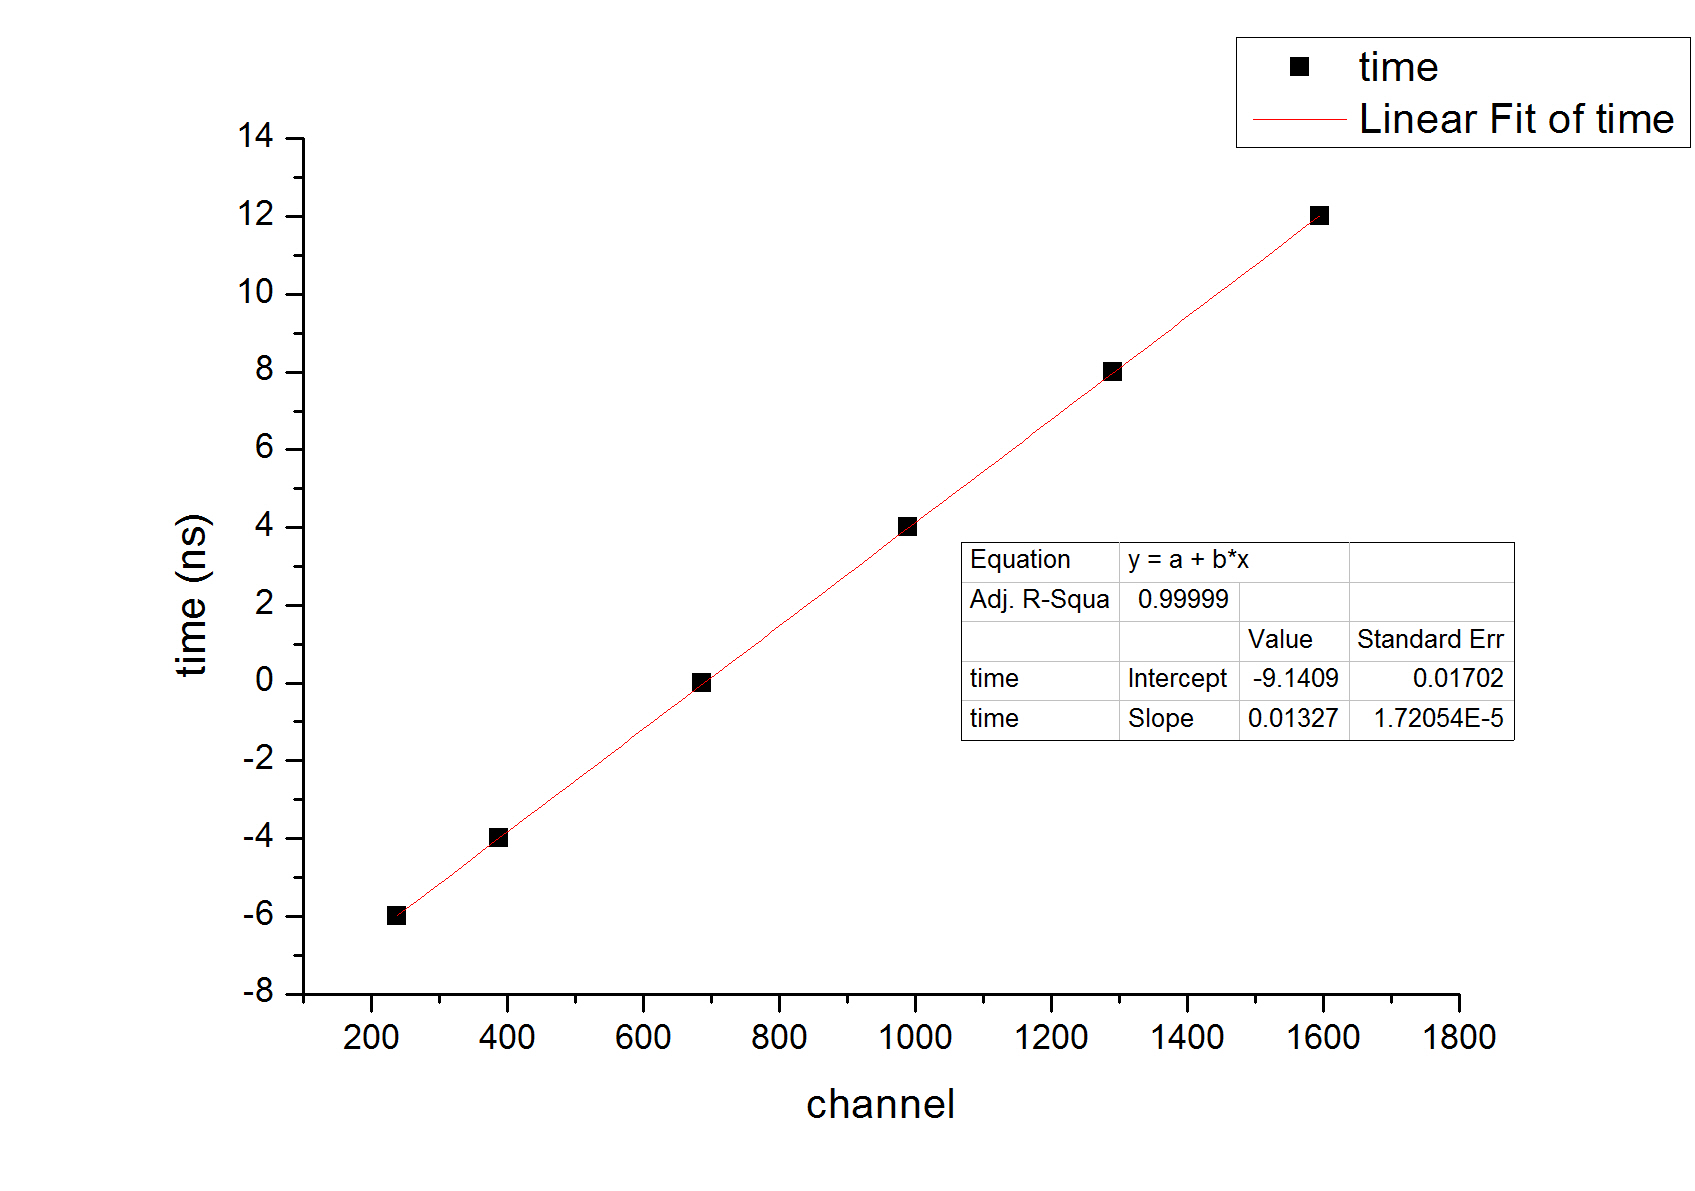
\includegraphics[width=15cm]{Graph1}
\caption{Linear fitting of channels and time}
\label{channel-time}
\end{center}
\end{figure}
\par
So we could substitute channel with time in the following data.

\section{Lifetime of D149}
With the data of liquid solution and solid state, the relative results could be obtained by convolution. Here is the result we obtained:\par
\begin{figure}
\begin{center}
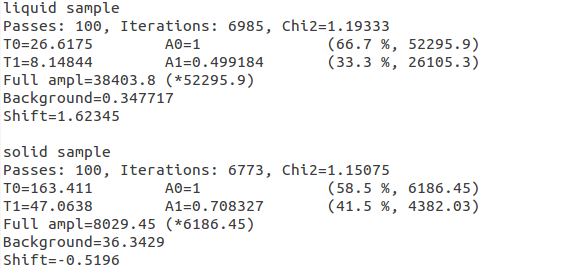
\includegraphics[width=10cm]{result1}
\caption{Results with convolution}
\label{convolution}
\end{center}
\end{figure}
\par
Here, time was in the scale of channel. If we multiple the data with the slope 0.0132, lifetime comes into ns scale, shown in Table \ref{my-label2}:
\par
\begin{table}
\centering
\caption{Life time of D146}
\label{my-label2}
\begin{tabular}{@{}lll@{}}
\toprule
States & Liquid & Solid\\ \midrule
time/channel  & 26.62 & 163.41 \\ 
time/ns &0.35 & 2.16 \\
\bottomrule
\end{tabular}
\end{table}




\section{Anistrotropy of Rhodamine 6G}
When the data of intensity-time of Rhodamine 6G in different direction (horizontal and vertical) are collected, anisotropy-time relations are obtained after treating them with Equation(\ref{r}).\par 

The original data are shown in Figure(\ref{r-time}).
\begin{figure}
\begin{center}
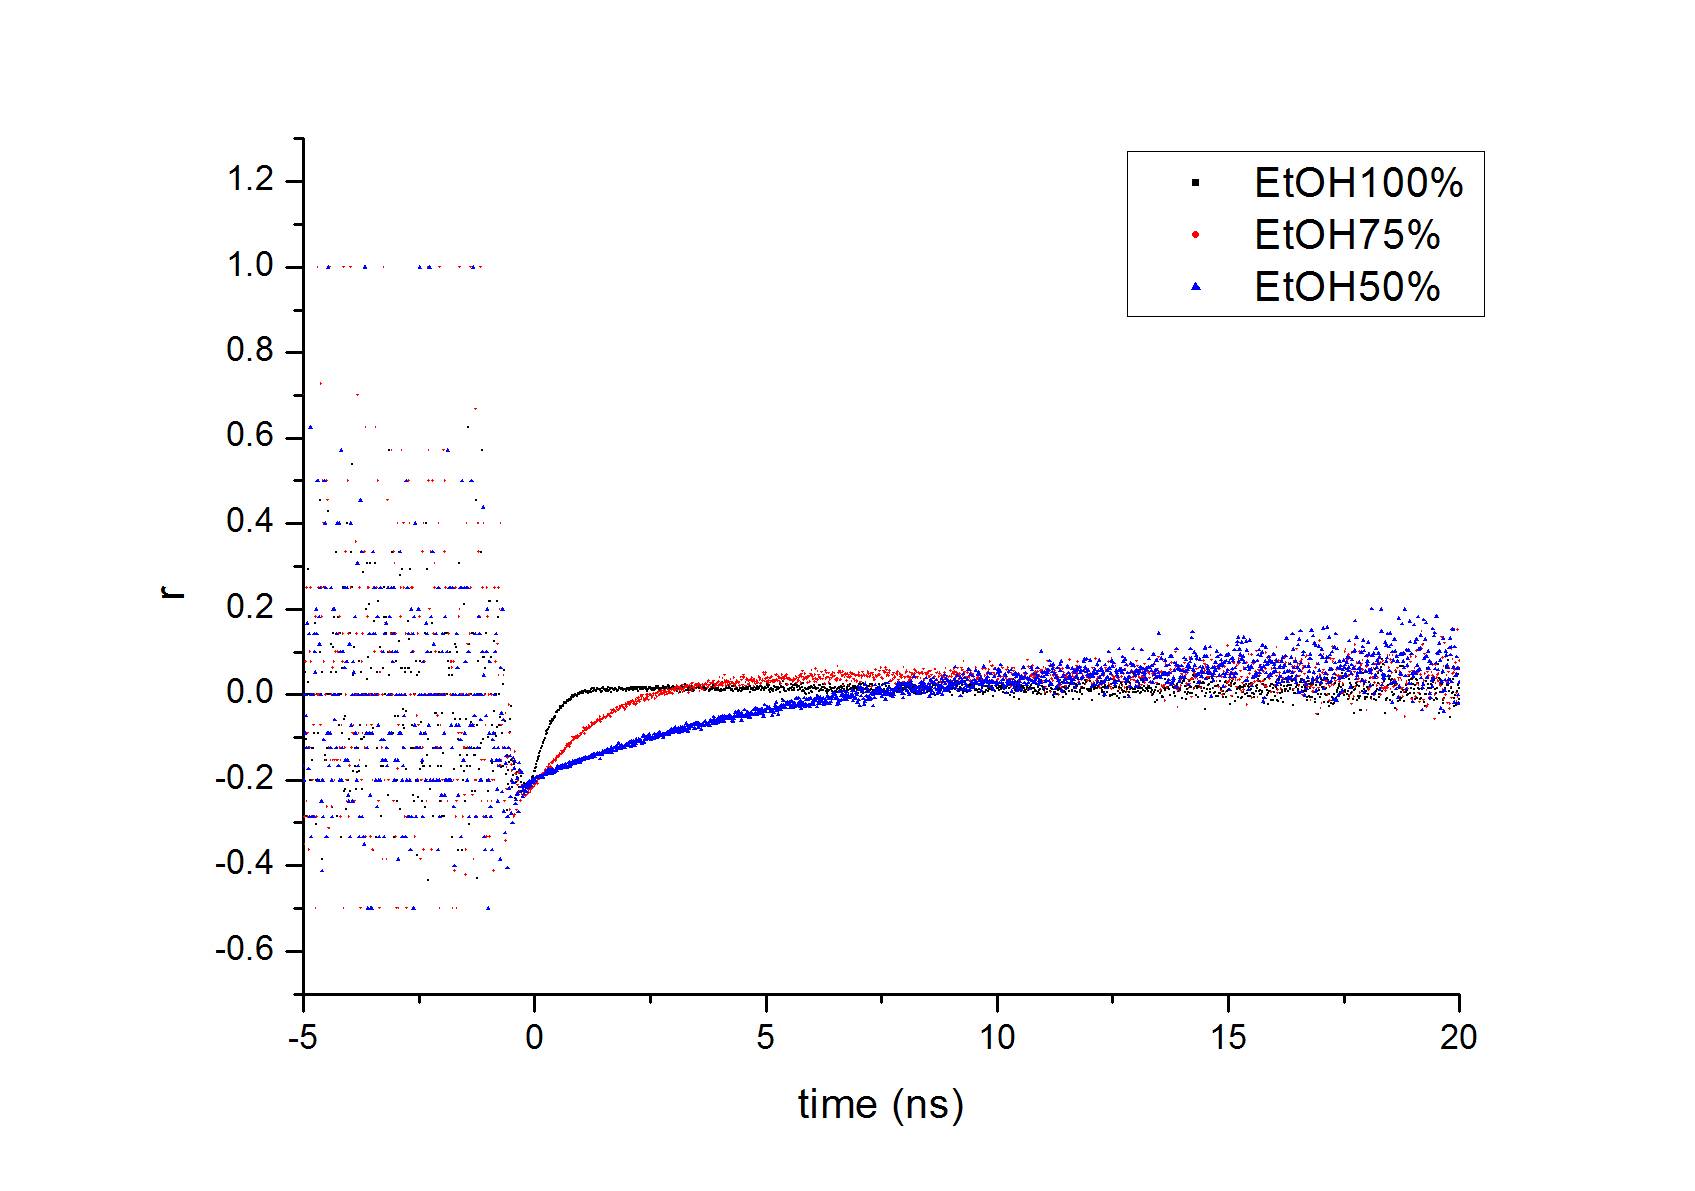
\includegraphics[width=15cm]{Graph3}
\caption{r-time relation of three solutions}
\label{r-time}
\end{center}
\end{figure}
\par 
Here can we observe that only after $t>0$, the molecule started to obey equation(\ref{r}). But after a long time, the fluctuation of signal is too large. Hence, I choose the time period $[0,15]$ns to do curve fitting with equation(\ref{r2}). \par

\begin{figure}
\begin{center}
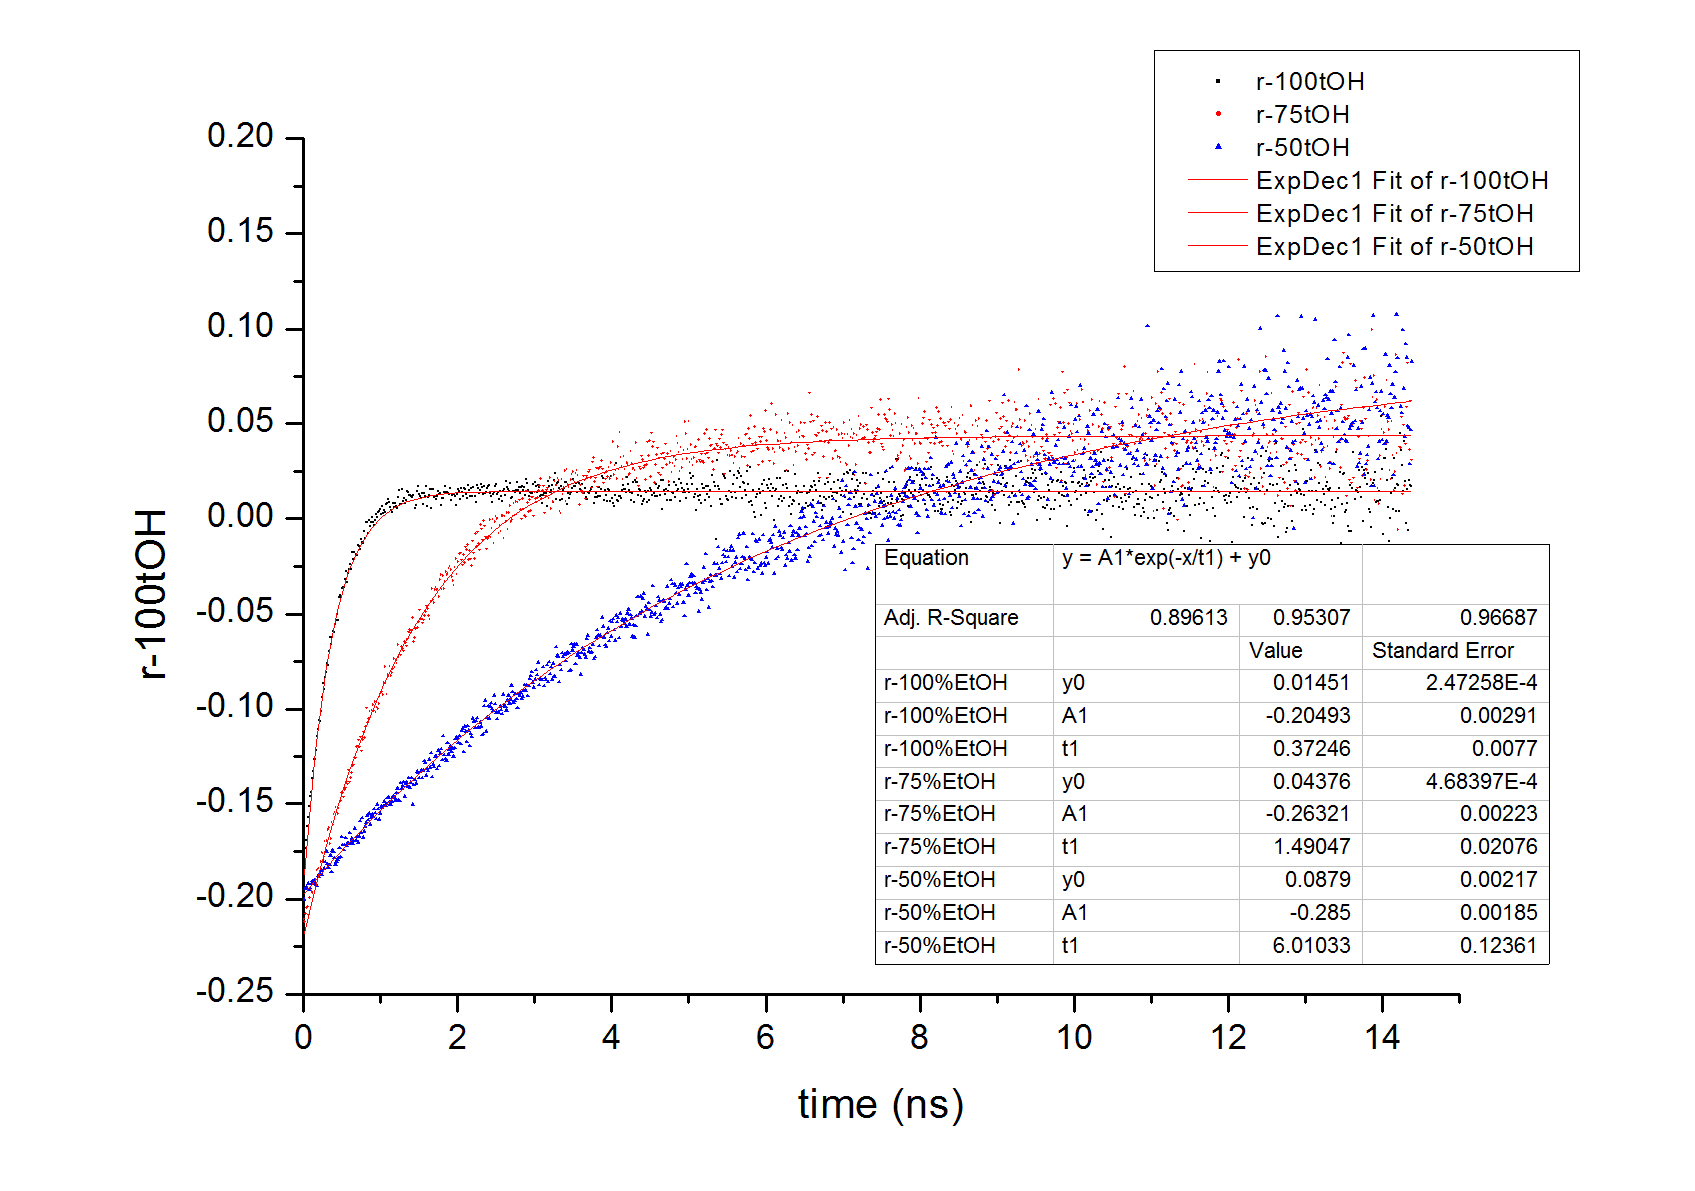
\includegraphics[width=15cm]{Graph2}
\caption{r-time fitting of three solutions}
\label{r-time-fitting}
\end{center}
\end{figure}
\par 
From the fitting results in figure(\ref{r-time-fitting}), we list the rotation correlation time $\theta$  in Table \ref{my-label3}.\par

\begin{table}
\centering
\caption{Rotation correlation time $\theta$}
\label{my-label3}
\begin{tabular}{@{}llll@{}}
\toprule
Liquid & 100\%EtOH & 75\%EtOH &50\%EtOH\\ \midrule
$\theta$/ns  & 0.372 & 1.490 &6.010\\ 
\bottomrule
\end{tabular}
\end{table}



\section{Questions}
1.  Imagine two compounds with similar fluorescence quantum yields (e.g. $\Phi_{fl} = 1$) but very different
absorption coefficients ($\varepsilon$). Now assume two samples of these with similar absorption (at a given
wavelength). What would be the difference between their time-resolved fluorescence spectra? Consider
the total fluorescence and how the fluorescence would be distributed over time.\\ \par 

Since the quantum yields are the same, when 2 samples have similar absorption, the exponential fluorescence spectra have similar integral area. According to 
\begin{equation}
A=\log (\frac{I_0}{I})=\varepsilon cl
\end{equation}
the larger absorption coefficients $\varepsilon$ means smaller life time $\tau$. To make sure the same integral area, the intial value of I becomes larger and the spectra decreases faster.\\ \par 


2.  What is the influence of laser intensity fluctuations (say within ±20\%) on the precision of the
measurement in a TCSPC life-time experiment? Compare that with an anisotropy measurement and with
fluorescence upconversion and transient absorption spectroscopy.\\ \par 
For life-time experiment, 20\% laser intensity flucturations do not influence the result becasue only 1\% intensity is measured for detection rather than the maximum value of the pulse.\par 
For anisotropy measurement, it influences the experiment results because we should do summation and subtraction on different intensity values in different measure direction(vertical or horizontal). In fluorescence upconversion, it does't matter because average intensity are detected. \\ \par 

3. Discuss the different lifetimes that were obtained during the measurement for the different systems,
taking into account the environments. \\ \par 

From the results in Table \ref{my-label2}, the lifetime of D149 in solid state(2.16ns) is larger than that in liquid solution(0.35), which arises from the solid state restriction of the motion of D149.\\ \par 

4. Estimate the volume of rhodamine 6G in three different ways: a) use the (estimated) density and
molecular mass and calculate the volume, b) estimate the diameter of the molecule by assuming standard
bond lengths and calculate the corresponding volume if it was a sphere (how realistic is that model?), c)
calculate the volume based on the time-resolved data in ethanol.
Compare the three ways and comment on which you consider most reliable. \\ \par 
a) 
\begin{equation*}
V=\frac{m}{\rho}=\frac{479.02 g/mol}{1.26 g/cm^3\times 6.623\times 10^{23}/mol}=0.574 nm^3
\end{equation*}
b) Diameter is about 12 C-C bonds length, which is 0.154 nm.  
\begin{equation*}
V=\frac{4\pi r^3}{3}=\frac{4\times 3.14\times 0.077^3}{4}=1.91\times 10^{-3} nm^3
\end{equation*}
c) In 100\% EtOH, $\theta = 0.372ns$. From equation(\ref{r2}),
\begin{equation}
V= \frac{\theta RT}{\eta} =\frac{0.372\times 10^{-9} \times 8.314 \times 298.15}{1.074\times 10^{-3}\times 6.023\times 10^{23}} m^{3}=1.426 nm^3
\end{equation}  
The second calculation is obviously wrong because molecules stay at a certain distance where their potential is zero in equilibrium. If we only take the distance of bond lengths into account, molecules must be at a great repulsion since they are so close to each other. Hence this result is smaller than other approximation results. \\ \par 

5. Based on the SPC data, calculate the rotational correlation time of rhodamine 6G in ethanol and
ethanol/glycerol. Also, calculate the viscosity of the mixtures and compare to the calculated viscosity based on a simple linear interpolation between those of the two pure solvents. \\ \par
Rotational correlation time is list in Table \ref{my-label3}. \par 
If we calculation viscosity from equation(\ref{r2}), we should determine the volume of molecule as $1.426 nm^3$ that I mentioned in question 4(c). The results of viscosity are shown in table 
\ref{my-label4}. The difference of viscosity that calculated from different ways are extremely large when glycerol is added to the solution, which reveals the non-ideal property of ethanol/glycerol solution ---we can not deals them as ideal solution and the viscosity of mixed solution can not be added simply. \\ \par

\begin{table}
\centering
\caption{Different viscosity}
\label{my-label4}
\begin{tabular}{@{}llll@{}}
\toprule
Liquid & 100\%EtOH & 75\%EtOH &50\%EtOH\\ \midrule
$\theta$ from TCSPC/ns  & 0.372 & 1.490 &6.010\\ 
Viscosity  & 1.074 & 4.302 &17.34\\ 
Linear viscosity calculation(298K)  & 1.074 & 234.3 &467.5\\ 
\bottomrule
\end{tabular}
\end{table}


6.  Given a new molecule with completely unknown photophysics/-chemistry, suggest a good strategy on
how to learn about possible processes that the molecule can undergo. Suggest possible techniques (flashphotolysis,
SPC, pump-probe, upconversion, streak camera, ...), why you use those and what you can
learn from these and what not (strengths and weaknesses). Keep in mind that practical aspects can be
quite important in many experiments. \\ \par


Given a new molecule, UV-vis and fluorescence emission spectra, which is extremely cheap and convenient, should be taken into account firstly. After these steps, we clearly know that if this molecule undergoes the $S_0 \rightarrow S_1$ or other transition at common wavelength range of light. And several state-to-state transition wavelength peaks are also obtained.\par 
After pump-probe, different photophysical/-chemical process are shown.  Then we obtain its lifetime of corresponding excited states with TCSPC measurement. Streak camera and upconversion are performed later.\\ \par
\end{document}
